

\documentclass[a4paper]{report}
\usepackage[margin=1in]{geometry}
\usepackage{polyglossia}
\setdefaultlanguage{danish}
\usepackage{titlepic}
\usepackage{graphicx}
\usepackage{xcolor}
\usepackage{amsfonts, amsmath, amssymb}
\usepackage{float} %ensures that figures / tables can be floated on page
\usepackage{fancyref}
\usepackage[sorting=none,backend=biber]{biblatex}
\usepackage{notoccite}
\addbibresource{../references.bib}

\newcommand{\MATLAB}{\textsc{Matlab}}
\newcommand{\sbul}{\begin{itemize}}
\newcommand{\ebul}{\end{itemize}}


\usepackage{setspace}
\onehalfspacing % line spacing (is equal to baselinestretch 1.33)

\usepackage[numbered,framed]{matlab-prettifier}
\lstset{
  language           = Matlab,
  style              = Matlab-editor,
  basicstyle         = \mlttfamily,
  escapechar         = `,
  mlshowsectionrules = true
}

\usepackage[binary-units=true]{siunitx}
\sisetup{detect-all}

%\definecolor{vertmatlab}{RGB}{28,160,55}
%\definecolor{mauvematlab}{RGB}{155,71,239}
%\definecolor{fond}{RGB}{246,246,246}
\definecolor{lightgray}{gray}{0.7}

\sloppy
\setlength{\parindent}{0pt}

\usepackage{titlesec}
\titleformat{\chapter}{\huge\bf}{\thechapter.}{20pt}{\huge\bf}
\titleclass{\chapter}{straight}

\usepackage[colorlinks,citecolor=blue,linkcolor=black,urlcolor=blue]{hyperref}

\author{Janus Bo Andersen \thanks{ja67494@post.au.dk}}
\titlepic{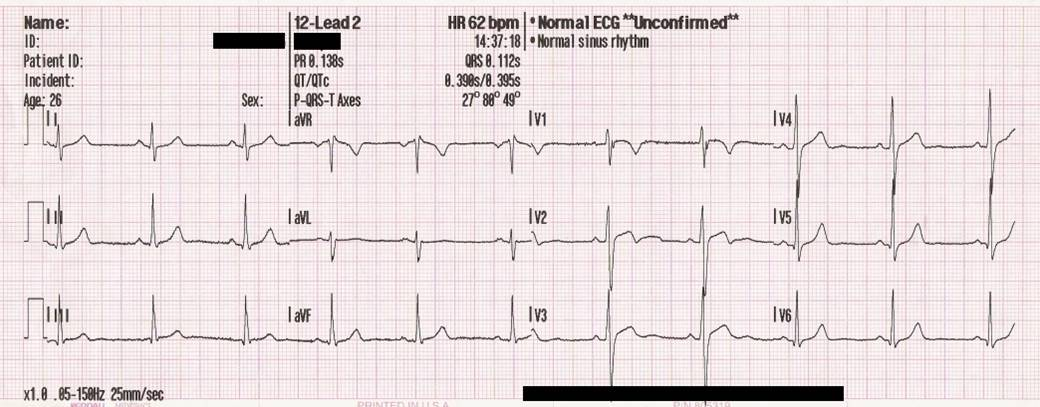
\includegraphics[width=\textwidth]{../img/12leadECG.jpg}}


\begin{document}

\pagenumbering{roman}


    
    
    \title{E3DSB miniprojekt 4 - Digital signalbehandling af elektrokardiogrammer}
        

    \maketitle

\tableofcontents
\newpage

\pagenumbering{arabic}

    \begin{par}

\chapter{Indledning}
Fjerde miniprojekt i E3DSB er frit og udarbejdet individuelt med teori og metoder fra hele kurset.
Ud over E3DSB er der bl.a. fundet inspiration til projektet i ST2PRJ2 fra ASE \cite{st2prj2}.

\end{par} 
\begin{par}

\section{Valgt emne}
Elektrokardiografi er medicinsk signalbehandling til at måle et hjertes elektriske aktivitet.
Signalet behandles først analogt og så digitalt for at danne et elektrokardiogram (EKG).
EKG'er bruges til at screene, diagnosticere og monitorere hjertepatienter, og fx til råd og vejledning i hjertestartere.
\\ \\
EKG'er er interessante, fordi analysemetoderne fra E3DSB er velegnede.
Der er meget information i både tids- og frekvensdomænet for et EKG-signal.
Der er desuden støj og andre signalkomponenter, der skal filtreres bort, samt udfordrende tekniske problemstillinger.

\end{par} 
\begin{par}

\section{Formål, metode og struktur}
Projektet demonstrerer, hvordan værktøjer fra E3DSB i \MATLAB~kan anvendes på EKG-signaler.
Dvs. hvordan information udtrækkes fra EKG-signalet i både tids- og frekvensdomænet.
Metoden er at sammenligne resultater fra raske (kontrolgruppe) og diagnosticerede patienter (ekspertvurdering).
Fokus er på arytmier.
\\ \\
\textbf{Analyse} redegør kort for EKG-signalet og anvendelser.
\textbf{Design} udarbejder og karakteriserer filtre.
\textbf{Implementering og test} demonstrerer analyser på EKG-signaler fra raske og sammenligner med diagnosticerede patienter.
En del kode er implementeret i hjælpefunktioner, som ses til sidst i~\textbf{\nameref{sec:hjfkt}}.
Følgende figur opsummerer flow for signalbehandlingen.
\begin{figure}[H]
\centering
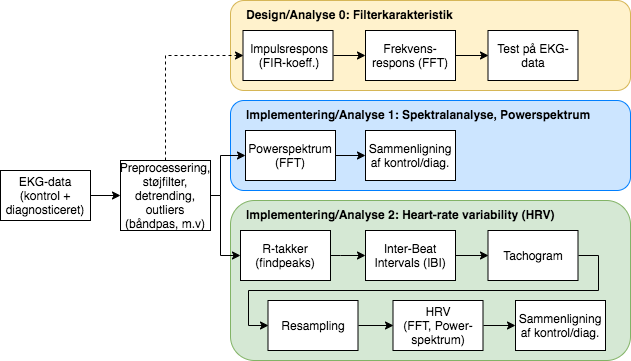
\includegraphics[width=14cm]{../img/minipro4.png}
\caption{Design og implementering\label{fig:design}}
\end{figure}

\end{par} 
\begin{par}

\section{Datakilder}
PhysioNet (\url{https://physionet.org/}) er et arkiv med medicinske, fysiologiske og biologiske signaler.
Der findes også gode værktøjer, og bl.a. ATM (\url{https://archive.physionet.org/cgi-bin/atm/ATM}) er nyttig til at finde og downloade data.
Projektet benytter derfra serier fra to datasæt.
Det simulerede signal er benyttet til eksperimenter og algoritmeudvikling ej inkluderet i rapporten.

\end{par} 
\begin{par}

\begin{table}[H]
\centering
\begin{tabular}{|p{1cm}|p{3cm}|p{6cm}|p{5cm}|} \hline
Kilde & Navn & Beskrivelse & Benyttede datasæt \\ \hline
\cite{ptb}
 & PTB Diagnostic ECG Database
 & Klinisk data fra 268 patienter i forskellige diagnostiske klasser
 & Pt.104, 116 (kontrol); Pt.113 (atrieflim.); Pt.126 (palpitation) \\ \hline
\cite{challenge2011}
 & PhysioNet Challenge 2011
 & Simuleret EKG-data til udvikling af computerbaseret diagnostik
 & Sim. \#2: Normal 80 BPM. Kun til udvikling. \\ \hline
\end{tabular}\caption{Datasæt benyttet i projektet}
\label{tab:datasets}
\end{table}

\end{par} 
\begin{par}

\section{Software, data og kildekode}
Rapport, databehandling og grafer er udarbejdet i \MATLAB{} R2018b update 5.
\TeX-kode er dannet fra \MATLAB-kode vha. en tilpasset XSL-template.
Lua\LaTeX{} er benyttet til at compile en PDF.
\MATLAB-kode, data og template findes på \url{https://github.com/janusboandersen/E3DSB}.

\end{par} 
\begin{par}

\chapter{Analyse}
Først opridses (kort) baggrund for EKG-signalet.
Så gennemgås et par indikationer og analysemetoder på relevante kardiovaskulære lidelser.
Endelig diskuteres problemer ifm. signalbehandling på EKG-data.

\end{par} 



\section{EKG-måling}

        \begin{par}

EKG'et tages med 10 elektroder på patientens krop:
4 placeres på arme og ben (ekstremiteter), 6 på brystkassen (thorax) \cite{absalon}.
Elektrisk potentiale måles mellem 12 forskellige kombinationer af elektroderne.
Hver kombination kaldes en \textbf{afledning}.
\begin{figure}[H]
\centering
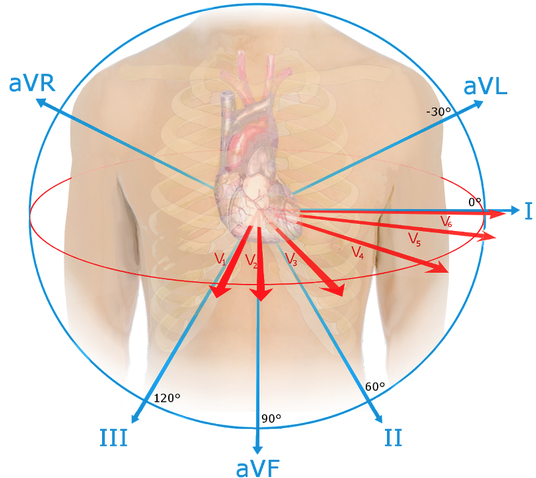
\includegraphics[width=5cm]{../img/ecg-lead-angles.png}
\caption{De 12 afledninger fra et EKG\label{fig:afledninger}}
\end{figure}
En afledning er et vektorsignal, som viser hjertets aktivitet i bestemt retning/vinkel.
Ovenstående figur illustrerer de 12 afledninger \cite{ecgbasics}.
I dette projekt benyttes kun \textbf{afledning-\texttt{II}}.
\texttt{II} giver det største signal, da måleretningen vektorielt er alignet med den længste akse i hjertet.
Dette er også udbredelsesretning for depolariseringsimpulsen, der giver hjertemuskulaturens sammentrækning,
samt for den følgende repolariseringsimpuls \cite[ca. 13m36s]{st2prj2}.

\end{par} 



\section{EKG-signalet}

        \begin{par}

Den elektriske impuls, der starter en hjertecyklus, udgår fra sinusknuden i højre forkammer (atrium).
Den normale hjerterytme kaldes derfor en sinusrytme.
En periode af signalet repræsenterer en hjertecyklus.
EKG'et viser flere ``takker'' og ``intervaller'', som har fysiologisk relevans.
Afstanden mellem flere følgende perioder afgør hjertets rytme.
Dette er illustreret i følgende figur \cite{realtimeecg}.
\begin{figure}[H]
\centering
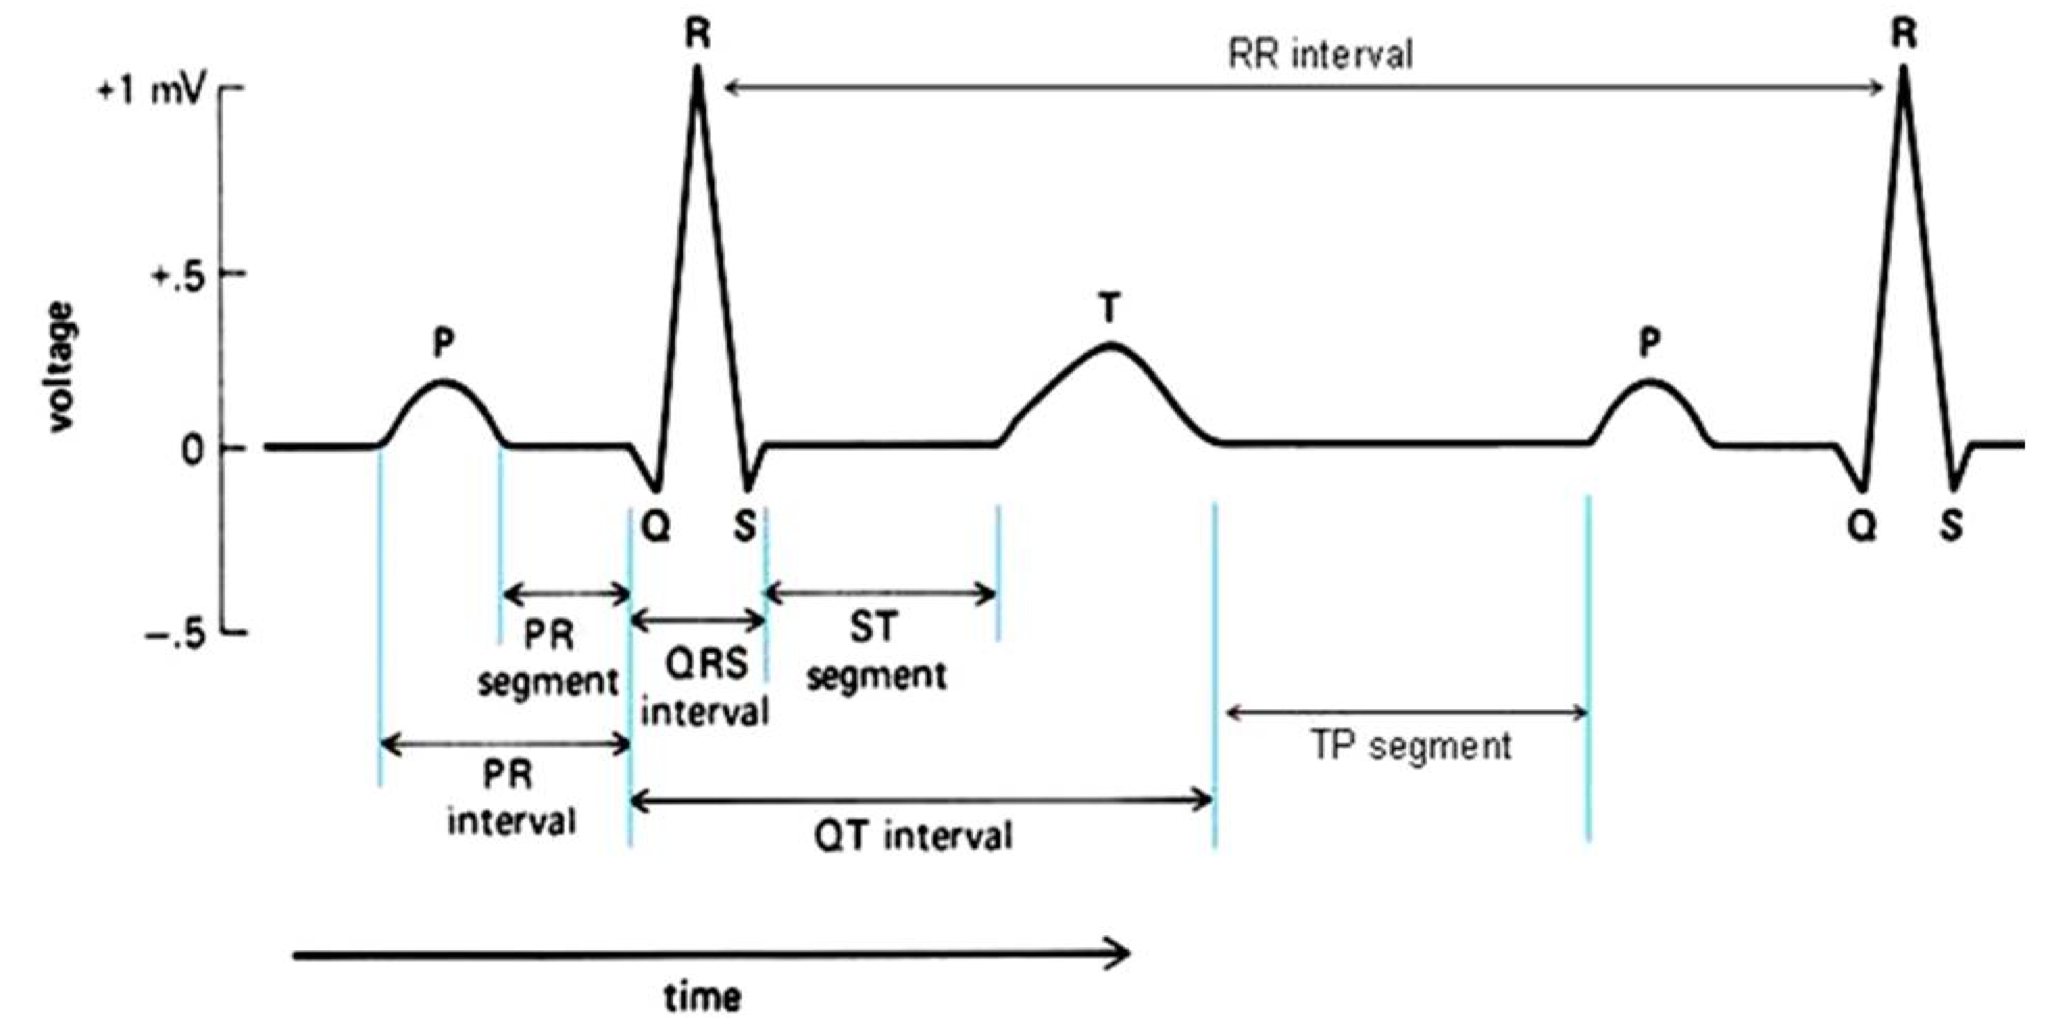
\includegraphics[width=14cm]{../img/ekg-graf.png}
\caption{EKG-signalets ``takker'' og ``intervaller''\label{fig:signal}}
\end{figure}
Hjertets sammentrækning (systole) begynder ved P-takken, hvor forkamrene (atrierne) trækker sig sammen.
Hjertekamrene (ventriklerne) trækker sig derefter sammen ved QRS-komplekset.
Her pumpes blod ud i kroppen.
R-takken er det højeste positive udslag i denne sammentrækning (for afledning-\texttt{II}).
T-takken viser ventriklernes repolarisering og start på hjertets afslapning og udvidelse (diastole) \cite{absalon}.
RR-intervallet måler afstanden i tid mellem to R-takker og kan bruges til at måle pulsen.
De flade linjesegmenter mellem takkerne kaldes baseline.
``Afstande'' og ``højder'' for forskellige komponenter har relevans i forskellige kliniske analyser.

\end{par} 
\begin{par}

\subsection{Hjerterytme, frekvenser og filtre}
EKG'er tages i hviletilstand, hvor pulsen ligger fra \SI{50}{\per\minute} til \SI{100}{\per\minute} \cite{absalonrytme}.
Alle signalkomponenter inden for en cyklus ligger derfor over \SI{0.8}{\hertz} (\SI{50}{\per\minute} omregnet).
Forventeligt ligger hvilepulsen omkring \SI{60}{\per\minute}, dvs. første komponent ved \SI{1}{\hertz}.
Harmoniske heraf vil også optræde.
Sygdomme kan tilføje mere højfrekvent flimren i signalet (se beskrivelse næste afsnit).
Klinisk udstyr bør kunne måle frekvenser i intervallet fra \SI{0.5}{\hertz} til \SI{150}{\hertz} for at opnå ``full fidelity'' \cite{emsfilter}.
Til dette projekt er der ikke behov for frekvenser over \SI{40}{\hertz}.
\\ \\
Sygdom kan give meget lav puls (brakykardi) eller meget høj puls (takykardi).
Pulsen kan da ligge fra \SI{30}{\per\minute} til \SI{300}{\per\minute}.
Det ligger dog udenfor analyserne i projektet.
\\ \\
Filtre kan nemt ødelægge information, der har klinisk relevans.
Så principielt bør alle filtre have lineær fase af diagnostisk grund (konstant group delay, ingen faseforvrænging).
\\ \\
Analyseformål og situation bestemmer de relevante frekvensbånd til analyse og støjfiltrering.
EKG-maskiner tilbyder forskellige filtre og indstillinger (monitorering, diagnostik, 50/\SI{60}{\hertz}, osv.).

\end{par} 



\section{Indikationer på hjerteproblemer og diagnostiske analyser}

        \begin{par}

Et EKG giver indikation på en række hjerteproblemer.
Her omtales kort hjerteproblemer relateret til arytmi (uregelmæssig rytme), som kan detekteres i et EKG-signal.
Afsnittet opridser to anvendte analyser med baggrund i metoder fra E3DSB.

\end{par} 
\begin{par}

\subsection{Arytmi}
Arytmi er uregelmæssig hjerterytme.
Det er normalt, at puls varierer med åndedræt (og fysiologiske processer).
Men det er unormalt, når pulsen varierer \textit{uregelmæssigt}, \textit{for meget} eller \textit{for lidt}.
Årsagerne til arytmi er mange, fx stress eller hjerteproblemer.
Konsekvenser varierer fra minimale til livstruende.

\end{par} 
\begin{par}

\subsubsection{Palpitationer}
En type arytmi er hjertebanken (palpitationer), der kan føles som om at hjertet springer slag over, eller slår for hurtigt.
I tidsdomænet er en indikation på arytmi, at det længste RR-interval er minimum \SI{0.16}{\second} længere end det korteste
\cite{st2prj2syg}\cite{bioelectric19}.
I en spektralanalyse vil arytmi give en bredere fordeling af energi i spektret, end tilfældet for en normal hjerterytme.

\end{par} 
\begin{par}

\subsubsection{Atrieflimren}
Atrieflimren (AF) (forkammerflimren, eng.: atrial fibrillation) er hyppigt, især hos ældre.
AF skyldes forstyrrelser i hjertets ledningsnet, og kan være følgelidelse til andre sygdomme.
Impulsen fra sinusknuden forlader ikke atriet, men cirkulerer rundt som en ``impulskarrusel'' \cite{absalonrytme}.
Så atriemuskulaturen laver mange sammentrækninger per pulsslag.
Atriefrekvensen er kraftigt forhøjet og uregelmæssig på mellem \SI{350}{\per\minute} og \SI{600}{\per\minute} \cite{atrieff}.
Pulsen svinger uregelmæssig mellem \SI{50}{\per\minute} og \SI{100}{\per\minute} \cite{absalonafli}.
\\ \\
Højfrekvente fluktuationer (flimrelinje) på baseline på EKG'et er et tegn \cite{absalonafli}.
Som ved palpitationer vil AF vise en bredere fordeling af energi i spektrum.
Det forventes, at der er mere energi ved højere frekvenser end er tilfældet ved palpitationer.

\end{par} 
\begin{par}

\subsection{Analyse 1: Powerspektrum}
Første analyse viser, hvordan energien i signalet fordeler sig som en funktion af frekvens.
Det relaterer til indikationer på arytmier fra forrige afsnit.
\\ \\
\textbf{Power-spektrum}: Power-spektrum beregnes via FFT'en.
Iflg. Parsevals sætning kan energi og effekt i tidsdomænet regnes fra Fourier-koefficienter i frekvensdomænet.
Gennemsnitseffekt for alle $N$ bins er:
$$ P = \frac{1}{N}\frac{2}{N}\sum_{k=0}^{N/2} X(k) \cdot X^*(k) $$
Her konjugeres frem for at kvadrere og tage modulus.
For at skalere FFT'en divideres med $N$.
For at regne effekt (ligesom $P=\frac{\Delta E}{\Delta t}$) divideres med $N$ igen.
Der skaleres med $2$ for at gå fra dobbeltsidet til enkeltsidet analyse (summationsgrænse $N/2$).

\end{par} 
\begin{par}

\subsection{Analyse 2: Heart-rate variability}
Heart-rate variability (HRV) giver et mål på pulsens variabilitet.
I litteraturen beskrives, at HRV bruges som risikomarkør for
kardiovaskulære sygdomme og for nervesystemets funktion \cite{taskforcehrv}.
HRV-analyser regnes klinisk fra EKG'et \cite{hrvhistory}.
Fitness-entusiaster kan se HRV på nyere pulsure og fitness-trackers.
HRV kan anskues både i tidsdomænet (statistisk) og frekvensdomænet.
Projektet fokuserer på frekvensdomænet.
\\ \\
HRV beregnes via spektralanalyse på længden af RR-intervallerne = IBI (inter-beat interval).
Visning af udviklingen af IBI over tid kaldes et tachogram.
Med et Powerspektrum på IBI (normaliseret) vises, hvor energien (variansen) er.
\\ \\
\textbf{Resampling og detrending:}
Pointen er at analysere den uregelmæssige rytme,
men metodisk er det en udfordring, at IBI-signalet er
samplet uregelmæssigt (en "sample" per pulsslag).
\MATLAB-funktionen \texttt{resample} bruges til at resample og
interpolere IBI-signalet til et regelmæssigt samplet signal med en højere
samplingsfrekvens \cite{resampling}.
Der vælges en ny samplingsfrekvens på 10 gange forventet pulsfrekvens.
Resampling stemmer overens med metodeanbefalinger \cite{taskforcehrv}.
IBI normaliseres til middelværdi på \SI{0}{\second}.
\\ \\
Litteraturen nævner mange mulige diagnostiske mål.
Et eksempel på et diagnostisk mål, der går igen flere steder, er \textbf{LF/HF}-ratioen for relativ energi i 2 frekvensbånd, hvor
\textbf{LF}-båndet er \SI{0.04}{\hertz} til \SI{0.15}{\hertz}, og \textbf{HF} er \SI{0.15}{\hertz} til \SI{0.4}{\hertz}.

\end{par} 



\section{Signalbehandling på EKG-data}

        \begin{par}

Påvirkning fra støj under målingerne giver uønsket påvirkning af EKG'et og det spektrale indhold.
Fysiologiske signaler har ``af natur'' variabilitet; dog er kun noget af variabiliteten brugbar.

\end{par} 
\begin{par}

\subsubsection{Støjkilder og støjfilter}
Der forventes en række støjartefakter ved opmåling af EKG:
\sbul
 \item Lavfrekvent støj fra patientens bevægelser og
  vejrtrækning (< \SI{50}{\per\minute} = \SI{0.8}{\hertz}).
 \item DC-støj fra kontaktpotentiale ved elektrode/hud-forbindelsen
  (op til 200-\SI{300}{\milli\volt}). Forværres af bevægelser og
  perspiration. \cite{emsfilter}.
 \item Baseline vandrer (driver) sfa. ovenstående el.lign. (ukendt frekvens).
 \item Muskelstøj i frekvensområdet 5-\SI{50}{\hertz}. Svært at filtrere \cite{emsfilter}.
 \item AC-støj fra elforsyning (\SI{50}{\hertz} i
    europæisk data og \SI{60}{\hertz} i amer.) samt harmoniske.
 \item Andre instrumenter og apparater i lokalet, fx mobiltelefoner.
\ebul
Der burde være common-mode-rejection via A/D-converteren, men elektroder
benyttet til opmåling er muligvis ikke ens, hvilket reducerer CMRR.
\\ \\
I projektet ignoreres frekvenser over \SI{40}{\hertz}, da der ikke er relevante fysiologiske komponenter.
Det tillader en simplificering af filteret til en lavere orden med bredere transitionsområde.
Dermed undgås også et båndstop-filter (notch), der skal flyttes alt efter datasættets oprindelsesland.
\\ \\
\textbf{Alt i alt:} Støjfilteret skal fungere som et \textbf{båndpasfilter},
der lukker frekvenser fra \SI{0.8}{\hertz} op til \SI{45}{\hertz} igennem
(regnet så der er \SI{5}{\hertz} transition op til powerline-støj, og \SI{5}{\hertz} ned til relevante frekvenser).
På den måde kan ovennævnte støjkilder frasorteres, og ``interessante'' frekvenser nævnt i tidligere afsnit stadig passere.

\end{par} 
\begin{par}

\subsubsection{Periodicitet og stationaritet}
DFT'en (FFT'en) er non-parametrisk, og forudsætter at signalet er én periode af et periodisk signal.
EKG-signalet er en \textit{ikke}-stationær proces og er ikke periodisk.
Fordelingsegenskaber er ikke stabile over tid, og amplitude, frekvens og fase vil ikke være konstante over tid.
\\ \\
Ikke-periodicitet håndteres med \textbf{vinduesfunktioner} i filterdesign og FFT'er for at få bedre kontrol over leakage og ripples.
\\ \\
Ikke-stationaritet gør fortolkning sværere, når en fysiologisk komponent optræder i flere bins pga. variation over tid.
I dette projekt gøres ikke noget for at håndtere dette.
En mulig metode er et glidende vindue, hvor signalsektioner analyseres separat.
Short-Time Fourier Transform (STFT) er et bud.

\end{par} 
\begin{par}

\chapter{Design}

\end{par} 
\begin{par}

\section{Filterdesign og pre-processering}
Filterbehov blev diskuteret tidligere.
Her designes og karakteriseres filter og pre-processering.
\\ \\
Støjfilteret er FIR-typen og har cut-off-frekvenser ved hhv. \SI{0.8}{Hz} og \SI{45}{Hz}.
Filteret skal have gain på \SI[per-mode=symbol]{1}{\volt\per\volt} i pasbåndet.
Der benyttes et Hann-vindue for at få hurtig transition og smal main lobe.
``Prisen'' er, at sidelobe-dæmpning ``kun'' er omkring -50 dB for de første par bins.
\\ \\
For at få et hurtigt roll-off, og dæmpning på \SI{6}{\decibel} ved \SI{0.8}{Hz}, skal filterorden for et højpasfilter være omkring 2000.
Så båndpas er designet som 2000.-ordens højpas foldet med et 200.-ordens lavpas.
\\ \\
Modsat et realtidssystem \textit{behøver} filtrene i projektet ikke at være kausale.
FIR-filtre designet efter metoder fra E3DSB er dog kausale.
For at undgå høj filterorden kunne ``forward-backward-filtering'' (IIR) give samme eller bedre respons med lavere filterorden og med zero-phase.
Et alternativ kunne være at fjerne lavfrekvente støjkomponenter med cubic-splines i tidsdomænet i stedet for at filtrere.
Begge dele dog udenfor projektets omfang.
\\ \\
Filteret fjerner gennemsnitligt DC-niv., men baseline er på medianen.
Så efter filtrering justeres DC-niveauet yderligere så baseline rykkes til \SI{0}{\milli\volt}.
\\ \\
Endelig fjernes outliers, her primært indsvingning (transiente) indtil delay-line er fyldt op.
\\ \\

\end{par} 

\begin{lstlisting}[language=Matlab, style=Matlab-editor]
clc; clear all; close all;
\end{lstlisting}
\begin{par}
Specificér og byg filteret og se impuls- og frekvensrespons. Alle dataserier har 1000 Hz samplingsfrekvens.
\end{par} 

\begin{lstlisting}[language=Matlab, style=Matlab-editor]
Fs = 1000;  % Hz          ord.  Fc   ord. Fc
h = ecg_noise_filter(Fs, [2000 0.8], [200 45]); % Som specificeret

% Respons i 4096-punkts FFT, 0-50 Hz på frek. akse, impulsresp. 1000-1200
show_filter_response(h, 4096, Fs, [0 50], [1000 1200]);
\end{lstlisting}

\begin{center}
    \includegraphics [width=5in]{miniprojekt_4_01.eps}
\end{center}
\begin{par}
Filterets pasbånd er som ønsket, og der er lineær fase. Impulsrespons viser, at efter ca. 1200 samples vil indsvingning af filter næsten være færdig (resterende koefficienter ``tæt på'' 0).
\end{par} 
\begin{par}

\section{Test af filter og pre-processering}
Filteret testes på kontrolgruppen.
Data loades og behandles, bl.a. justeres til rå værdier (data er lagret
med gain \SI[per-mode=symbol]{2000}{\volt\per\volt}). Der oprettes også
hjælpeserier i objektet (\texttt{ecg} er en \texttt{struct}).

\end{par} 

\begin{lstlisting}[language=Matlab, style=Matlab-editor]
A = 2000; B = 0;

% Patient 104: Kontrol (rask), mand 58, 60 s data, Fs=1000, A=2000, DC=0
ecg_ktr1 = ecg_load('data/kontrol/ktr1/s0306lrem.mat', 'Ktrl.1 (m/58)', ...
    'II', 'mV', A, B, Fs);

% Patient 116: Kontrol (rask), mand 54, 60 s data, Fs=1000, A=2000, DC=0
ecg_ktr2 = ecg_load('data/kontrol/ktr2/s0302lrem.mat', 'Ktrl.2 (m/54)', ...
    'II', 'mV', A, B, Fs);

d = {ecg_ktr1, ecg_ktr2};               % Gem på en smart måde til senere
\end{lstlisting}
\begin{par}
Pre-processér de to dataserier: Filtrér med støjfilter. Fjern indsvingning (fjernelse af første 1200 samples koster 1.2 sek. data). Justér baseline til 0 mV. Sammenlign før/efter-plots.
\end{par} 

\begin{lstlisting}[language=Matlab, style=Matlab-editor]
crop_samples = 1200;           % de første 1200 samples fjernes (indsv.)

for e=1:2
    d{e} = ecg_filtered_cropped_moved(d{e}, h, crop_samples);
end
ecg_show_processing( d(1:2) );        % Sammenlign før/efter
\end{lstlisting}

\begin{center}
    \includegraphics [width=5in]{miniprojekt_4_02.eps}
\end{center}
\begin{par}
Pre-processering virker som ønsket. Lavfrekvent støj og vandring på baseline fjernes. Signalets baseline ligger på 0 mV efter justeringer.
\end{par} 
\begin{par}

\newpage
\chapter{Implementering og test}
I dette afsnit implementeres Analyse 1 og Analyse 2.
Data for diagosticerede patienter loades og pre-processeres først.

\end{par} 

\begin{lstlisting}[language=Matlab, style=Matlab-editor]
% Pt. 126: Sinusarytmi: Hjertebanken, mand 62, 38 s, Fs=1000, A=2000, DC=0
d{3} = ecg_load('data/arytmi/sa/s0154_rem.mat', 'Palpitat. (m/62)', ...
    'II', 'mV', A, B, Fs);

% Pt. 113: Arytmi: Atrieflimren, kvinde 65, 38 s, Fs=1000, A=2000, DC=0
d{4} = ecg_load('data/arytmi/af/s0018crem.mat', 'Atrieflim. (k/65)', ...
    'II', 'mV', A, B, Fs);

for e = 3:4      % Pre-processer signaler for de to diagnosticerede pat.
    d{e} = ecg_filtered_cropped_moved(d{e}, h, crop_samples);
end
ecg_show_processing( d(3:4) );            % Sammenlign før/efter
\end{lstlisting}

\begin{center}
    \includegraphics [width=5in]{miniprojekt_4_03.eps}
\end{center}
\begin{par}
Igen bekræftes grafisk, at filtrering og anden pre-processeringen er gået OK.
\end{par} 
\begin{par}

\section{Analyse 1: Powerspektrum}
Analyse 1 udføres ved at regne powerspektra på de 4 serier, som beskrevet i analyseafsnittet.
FFT'en regnes med et Hann-vindue.
Med smoothing fås et lidt pænere spektrum (tak for funktionen, KPL!).
Endelig sammenlignes de resulterende spektra grafisk.

\end{par} 

\begin{lstlisting}[language=Matlab, style=Matlab-editor]
MA = 5;               % Smoothing af Powerspektrum glidende over MA bins
for e = 1:4           % Udfør for alle 4 serier
    d{e} = ecg_powerspectrum(d{e}, MA);
end
ecg_plot4_powerspectrum(d, [0 40]);         % Vis Powerspectrum fra 0-40 Hz
\end{lstlisting}

\begin{center}
    \includegraphics [width=5in]{miniprojekt_4_04.eps}
\end{center}
\begin{par}

Den først spike i spektret repræsenterer patientents puls (for de raske, i hvert fald).
For Ktrl.1 ligger den omkring \SI{1.05}{\hertz}.
Det svarer til en normal hvilepuls på \SI{63}{\per\minute}.
Ktrl.2 har puls omkring \SI{61}{\per\minute}.
\\ \\
Det ses, at spektra for kontrolgruppe og diagnoser er væsentligt forskellige.
For raske patienter ligger det meste af energien under \SI{10}{\hertz} i et pænt mønster af puls og harmoniske.
For Ktrl.2 ses der dog antageligt noget muskelstøj i området 10-\SI{30}{\hertz}.
\\ \\
Spektra for palpitationer og atrieflimmer svarer til forventningen fra teoriafsnittet om arytmier:
Der er \textit{væsentligt} bredere fordeling af energi i spektra for patienter med diagnose end for kontrolgruppen.
Der er intet pænt mønster af puls og harmoniske.
Atrieflimren har, som forventet, den bredeste fordeling.
\\ \\
Analysen demonstrerer, hvordan powerspektra kan bruges til give indikationer på hjertelidelser.
Spektra viser også, at der ikke er meget energi i båndet 30-\SI{40}{\hertz}.

\end{par} 
\begin{par}

\section{Analyse 2: Heart-rate variability}
HRV-analyse kræver i princippet mere end 4 minutters observationer for at kunne give valide data på relevante dele af spektre \cite{wikihrv}.
EKG-signalerne valgt til dette projekt (mellem 38-60 s lange) er principielt ikke lange nok til at give håndfaste estimater.
Men det er ok til at demonstrere analysen.
\\ \\
Med det ``in mente'' udføres Analyse 2 med baggrund i teoriafsnittet.
Først detekteres R-takkerne, og resultatet inspiceres grafisk.
For at detektere R-takker algoritmisk, sættes der en tærskelværdi manuelt.
Den er sat ved inspektion af tidsserierne (ca. hvilket niveau i signalet overstiges kun af R-takker).
Der kunne også findes automatiske metoder.
\MATLAB's \texttt{findpeaks} benyttes til at lokalisere peaks.
Kriteriet er: En peak er en sample med højere værdi end sine to naboer og over tærskelværdien.
RR-intervallerne og IBI (normaliseret, i sek.) beregnes derefter.

\end{par} 

\begin{lstlisting}[language=Matlab, style=Matlab-editor]
thresholds = [0.5, 0.5, 0.17, 0.25];    % Tærskelværdier per inspektion, mV

for e = 1:4                 % R-takker og IBI-intervaller for alle 4 serier
    d{e} = ecg_find_r_ibi(d{e}, thresholds(e));
end
ecg_plot4_peaks(d, [0 60]);             % Vis R-takker for serierne, 0-60s
\end{lstlisting}

\begin{center}
    \includegraphics [width=5in]{miniprojekt_4_05.eps}
\end{center}
\begin{par}

Diagrammerne bekræfter, at algoritmen har detekteret alle R-takkerne ud fra de givne tærskelværdier.
Der vises også beregnet puls over hele serien, som svarer fint til beregninger baseret på frekvenser i Powerspektrum.
Hjerterytmen for diagnosticerede patienter virker, helt forventeligt, ud fra diagrammet mere variabel og ``kaotisk'' end for de raske kontroller.
Bemærk, at patienten med atrieflimren har en forhøjet puls.
\\ \\
Tachogrammerne vises for at illustrere udsving ift. det gennemsnitlige inter-beat interval.

\end{par} 

\begin{lstlisting}[language=Matlab, style=Matlab-editor]
ecg_plot4_tachogram(d);
\end{lstlisting}

\begin{center}
    \includegraphics [width=5in]{miniprojekt_4_06.eps}
\end{center}
\begin{par}

Tachogrammerne viser ret tydeligt, at der er forskel på variabilitet i hjerterytmen hos raske versus diagnosticerede,
især for patienten diagnosticeret med atrieflimren. Sammenlign fx mindste
og højeste værdi for IBI - i serien for palpitationer, er der mere end
\SI{0.6}{\second} i forskel mellem korteste og længste interval.
For de raske patienter ses også variabilitet.
Her er det overvejende mest sandsynligt, at størstedelen er drevet af vejrtrækningen, hvilket er helt normalt.
Hjerterytmen har høj korrelation med respirationen, hvilket kaldes respiratorisk sinusarytmi (RSA).
Variansen ($\sigma^2$) for hver serie er angivet i diagrammet.
Igen bekræftes, at de diagnosticerede har højest varians i hjerterytmen.
\\ \\
Fra tachogrammet ``føles'' det nærliggende at lave en spektralanalyse.
Det er tydeligt fra figurer, at samplingen har været uregelmæssig.
Først skal IBI-serien resamples \cite{resampling}.
\\ \\
Afstanden i tid mellem hver sample er givet fra
\texttt{findpeaks}-algoritmen.
Splines-metoden benyttes til at interpolere mellem samples, fordi
standardmedoden slet ikke kan fange al variabiliteten i IBI-signalet.

\end{par} 

\begin{lstlisting}[language=Matlab, style=Matlab-editor]
%        Gns. puls for     K1 K2 SA AF
desiredFs = round((10/60)*[61 60 72 103]); % 10 x gennemsnitspuls i Hz
                                           % som omtalt i teoriafsnit
for e = 1:4
    d{e} = ecg_ibi_resample(d{e}, desiredFs(e));    % Resample hvert IBI
end
ecg_show_resampling(d);                    % Vis resultater af resampling
\end{lstlisting}

\begin{center}
    \includegraphics [width=5in]{miniprojekt_4_07.eps}
\end{center}
\begin{par}

Resultatet af resamplingen virker overordnet fornuftigt, bortset fra at
den resamplede serie for palpitationer har lidt afvigelse omring 21-\SI{25}{\second}.
\\ \\
HRV-analysen regnes med de nye regelmæssigt samplede serier.
Powerspectrum beregnes, og samtidig regnes LF/HF-ratioen.
Der benyttes \textit{ikke} et Hann-vindue i denne FFT.
Powerspectrum udglattes til brug i grafer ved et glidende gennemsnit.
\\ \\
HRV-analysen er primært relevant i frekvensområden 0-\SI{0.5}{\hertz}.
Specifikt kigges på intervallerne LF: 0.04-\SI{0.15}{\hertz} og
HF: 0.15-\SI{0.4}{\hertz}. Disse intervaller er markeret i diagrammet.
Et udglattet powerspectrum plottes, og beregnede
LF/HF-ratioer er vist for hver patient.
\\ \\

\end{par} 

\begin{lstlisting}[language=Matlab, style=Matlab-editor]
MA = 5;               % Smoothing af Powerspektrum glidende over MA bins
for e = 1:4
    d{e} = ecg_hrv_powerspectrum(d{e}, MA);  % Beregn HRV for hver patient
end
ecg_plot4_hrv(d, [0 0.5]);                   % Vis HRV for f op til 0.5Hz
\end{lstlisting}

\begin{center}
    \includegraphics [width=5in]{miniprojekt_4_08.eps}
\end{center}
\begin{par}

Som nævnt i indledningen til analysen lider resultatet under at
dataserierne er relativt korte.
Desuden er der mange forskelllige mulige diagnostiske grænser for LF/HF.
Ikke desto mindre er det interessant at observere,
at begge kontroller har LF/HF $> 1$, mens de to diagnosticerede
patienter har LF/HF $< 1$.
Det fremgår således, at energien i nervesystemets impulser er
mere højfrekvent for de to diagnosticerede patienter, relativt til
kontrollerne.
\\ \\
Denne analyse har vist, hvordan Fourieranalyse kan benyttes til at
implementere en nyere diagnostisk teknik. Længere dataserier ville
give analysen mere kraft.

\end{par} 
\begin{par}

\chapter{Konklusion}
Denne rapport har demonstreret metoder fra E3DSB anvendt på EKG-signaler.
Det er vist, hvordan information, som kan have diagnostisk relevans for
sundhedspersonale, fx kardiologer, udtrækkes fra EKG-signalet i
tids- og frekvensdomænet. Forbedringsforslag til metoder modtages meget gerne!
\\ \\
Projeket har også demonstreret, hvordan en lidt større datanalyse kan
gribes an i \MATLAB. Gode råd, tips og tricks modtages meget gerne.
Det fremgår nok af rapporten, at det var nødvendigt at bruge en del
tid på at oparbejde viden omkring fagområdet \textit{og}
bruge en del tid på at forbehandle data, før der egentlig kunne
udarbejdes analyser.

\end{par} 

\begin{par}

\newpage
\chapter{Implementerede hjælpefunktioner\label{sec:hjfkt}}
Der er til projektet implementeret en række hjælpefunktioner.

\end{par} 



\section{ecg\_noise\_filter}

        
\begin{lstlisting}[language=Matlab, style=Matlab-editor]
function [h] = ecg_noise_filter(Fs, highpass, lowpass)
% Lav et båndpasfilter. Specificér hp, lp koeff. som [orden Fc]
% Janus Bo Andersen, 2019
    flag = 'scale';               % Normaliser koeff. til pasbånd på 0 dB
    win_hp = hann(highpass(1)+1); % Vinduesfkt. af Hann-typen
    win_lp = hann(lowpass(1)+1);  % Ditto
    hp  = fir1(highpass(1), highpass(2)/(Fs/2), 'high', win_hp, flag);
    lp  = fir1(lowpass(1), lowpass(2)/(Fs/2), 'low', win_lp, flag);
    h = conv(lp, hp);             % Fold lavpas og højpas sammen
end
\end{lstlisting}



\section{show\_filter\_response}

        
\begin{lstlisting}[language=Matlab, style=Matlab-editor]
function [] = show_filter_response(h, N, Fs, flim, hlim)
% Viser filterrespons i dB
% Janus Bo Andersen, 2019
    setlatexstuff('Latex'); figure              % Figurindstillinger
    H = fft(h, N);                              % Frekvensrespons
    k = floor( flim(2)*(N/Fs) );                % Højeste bin vi vil se

    subplot(2,2,1:2)                            % Impulsrespons
    stem(hlim(1):hlim(2), h( hlim(1)+1:hlim(2)+1 ))
    xlabel('$n$', 'Interpreter','Latex', 'FontSize', 15);
    ylabel('Impulsrespons', 'Interpreter','Latex', 'FontSize', 15);
    grid on;

    subplot(2,2,3)                              % Amplituderespons
    plot((1:k)*(Fs/N), mag2db(abs(H(1:k))) );
    xlabel('$f$ [Hz]', 'Interpreter','Latex', 'FontSize', 15);
    ylabel('Amplitude [dB]', 'Interpreter','Latex', 'FontSize', 15);
    ylim([-40 5]);
    grid on;

    subplot(2,2,4)                              % Faserespons
    plot((1:k)*(Fs/N), angle(H(1:k))*180/pi );
    xlabel('$f$ [Hz]', 'Interpreter','Latex', 'FontSize', 15);
    ylabel('Fase [deg]', 'Interpreter','Latex', 'FontSize', 15);
    grid on;

    sgtitle('Filterkarakteristik', 'Interpreter', 'Latex', 'FontSize', 20);
end
\end{lstlisting}



\section{setlatexstuff}

        
\begin{lstlisting}[language=Matlab, style=Matlab-editor]
function [] = setlatexstuff(intpr)
% Sæt indstillinger til LaTeX layout på figurer: 'Latex' eller 'none'
% Janus Bo Andersen, 2019
    set(groot, 'defaultAxesTickLabelInterpreter',intpr);
    set(groot, 'defaultLegendInterpreter',intpr);
    set(groot, 'defaultTextInterpreter',intpr);
end
\end{lstlisting}



\section{ecg\_load}

        
\begin{lstlisting}[language=Matlab, style=Matlab-editor]
function [ecg] = ecg_load ( filename, name, lead, unit, gain, offset, Fs )
%load_ecg læser en fil og returnerer en datastruktur med ECG-data
%   filename: filnavn med (type .mat)
%   name: navn på dataserien (bruges i plots)
%   lead: afledning ('I', 'II', 'III', osv.)
%   unit: enhed ('mV')
%   gain: forstærkning i data (typisk 200-2000)
%   offset: 0 medmindre der er benyttet anden base end 0
%   Fs: samplingsfrekvens
% Janus Bo Andersen, 2019

    ecg = load(filename, 'val');
    ecg.meta.name = name;               % Dataseriens navn
    ecg.meta.lead = lead;               % Benyttet afledning (I, II, ...)
    ecg.meta.unit = unit;               % Værdienhed for ECG-måling
    ecg.meta.gain = gain;               % Gain i data (.info-fil)
    ecg.meta.offset = offset;           % Base i date (.info-fil)
    ecg.Fs = Fs;                        % Samplingsfrekvens (.info-fil)

    % Afledte beregninger
    ecg.Ts = 1/ecg.Fs;                  % Sampleafst. på 1/Fs [s]
    ecg.N = length(ecg.val);            % Antal samples
    ecg.resolution = ecg.Fs / ecg.N;    % Frekvensopløsning [Hz/bin]
    ecg.T = ecg.N * ecg.Ts;             % Samlet tid i sek
    ecg.n = (0:ecg.N - 1);              % Vektor til samplenumre
    ecg.t = ecg.n * ecg.Ts;             % Vektor til tidsakse

    % Rådata (rå mV før justeringer i lagret datasæt)
    ecg.raw = (ecg.val - ecg.meta.offset) ./ ecg.meta.gain;
end
\end{lstlisting}



\section{ecg\_filtered\_cropped\_moved}

        
\begin{lstlisting}[language=Matlab, style=Matlab-editor]
function [ecg] = ecg_filtered_cropped_moved(ecg, h, crop)
% Returnerer processeret ECG-objekt, samples der fjernes er 1:crop.
% Baseline flyttes fra median til 0 V.
% Janus Bo Andersen, 2019

    ecg.filt.filtered = filter(h, 1, ecg.raw);          % Filtrering

    ecg.filt.filtered = ecg.filt.filtered(crop+1:end);  % Cropping
    ecg.filt.N = length(ecg.filt.filtered);
    ecg.filt.T = ecg.filt.N * ecg.Ts;
    ecg.filt.n = (0:ecg.filt.N - 1);
    ecg.filt.t = ecg.filt.n * ecg.Ts;
    ecg.h = h;                                          % Gem filteret

    m = median(ecg.filt.filtered);                      % Flyt baseline
    ecg.filt.filtered = ecg.filt.filtered - m;
end
\end{lstlisting}



\section{ecg\_show\_processing}

        
\begin{lstlisting}[language=Matlab, style=Matlab-editor]
function [] = ecg_show_processing(d)
% Plotter 2x2 plot med før/efter pre-processering
% d indeholder 2 ECG-objekter
% Janus Bo Andersen, 2019
    setlatexstuff('Latex'); figure                  % Figurindstillinger
    for p = 1:2
        subplot(2,2,p)                             % Ubehandlet EKG
        plot(d{p}.t, d{p}.raw);
        xlabel('$t$ [s]', 'Interpreter','Latex', 'FontSize', 10);
        ylabel(['Signal pre', ' [', d{p}.meta.unit, ']'], ...
            'Interpreter','Latex', 'FontSize', 10);
        grid on;
        title(d{p}.meta.name, 'Interpreter','Latex', 'FontSize', 15)

        subplot(2,2,p+2)                           % Processeret EKG
        plot(d{p}.filt.t, d{p}.filt.filtered);
        xlabel('$t$ [s]', 'Interpreter','Latex', 'FontSize', 10);
        ylabel(['Signal post', ' [', d{p}.meta.unit, ']'], ...
            'Interpreter','Latex', 'FontSize', 10);
        grid on;
        title('Efter pre-processering:', ...
            'Interpreter','Latex', 'FontSize', 15)
    end
    sgtitle('Effekt af pre-processering', ...
        'Interpreter', 'Latex', 'FontSize', 20);
end
\end{lstlisting}



\section{ecg\_powerspectrum}

        
\begin{lstlisting}[language=Matlab, style=Matlab-editor]
function [ecg] = ecg_powerspectrum(ecg, smooth_bins)
% Regner Powerspectrum på pre-processeret ECG-data
% Benytter Hann-vinduesfkt. og smoothing af Powerspektrum
% smooth_bins: Antal bins, i glidende gennemsnit (skal være ulige)
% Janus Bo Andersen, 2019

    x = ecg.filt.filtered;
    N = length(x);
    w = hann(N);                              % Hann-vinduesfkt.
    X = fft(x.*w');                           % Windowed FFT
    P = 2*(X.*conj(X))/(N^2);                 % Power for hver frekv.sample
    ecg.filt.Ps = smoothMag(P, smooth_bins);  % Glidende gennemsnit
    ecg.filt.Ps_sw = ecg.resolution*smooth_bins;  % Bredde af smoothing, Hz
end
\end{lstlisting}



\section{ecg\_plot4\_powerspectrum}

        
\begin{lstlisting}[language=Matlab, style=Matlab-editor]
function [] = ecg_plot4_powerspectrum(d, flim)
% Plotter 2x2 figur med powerspektra, og sætter xlim = flim
% d indeholder 4 ECG-objekter
% Janus Bo Andersen, 2019
    setlatexstuff('Latex'); figure              % Figurindstillinger

    for p = 1:4
        subplot(2,2,p)                          % Plot figur nr. p
        plot((1:d{p}.filt.N/2)*(d{p}.Fs/d{p}.filt.N), ...
            d{p}.filt.Ps(1:d{p}.filt.N/2))
        xlim(flim)                              % Begræns udbredning i x
        xlabel('$f$ [Hz]', 'Interpreter','Latex', 'FontSize', 10);
        title(d{p}.meta.name, 'Interpreter','Latex', 'FontSize', 15)
        grid on;
        txt = ['Smooth.vindue: ', num2str(d{p}.filt.Ps_sw,2), '[Hz]'];
        yLimits = get(gca,'YLim');
        text(flim(2)*0.35, yLimits(2)*0.9, txt)
    end
    sgtitle('Powerspektra [$\propto$ V$^2$Hz$^{-1}$]', ...
        'Interpreter', 'Latex', 'FontSize', 20);
end
\end{lstlisting}



\section{ecg\_find\_r\_ibi}

        
\begin{lstlisting}[language=Matlab, style=Matlab-editor]
function [ecg] = ecg_find_r_ibi(ecg, threshold)
% Finder R-takker vha. findpeaks og tærskelværdi
% Janus Bo Andersen, 2019
    ecg.filt.R.threshold = threshold;            % Gem tærskelværdi
    [ecg.filt.R.pk, ecg.filt.R.lk] = ...         % R Peakværdi og Lokation
        findpeaks(ecg.filt.filtered, ...         % Find i filtreret data
        ecg.Fs, 'MinPeakHeight', threshold);

    ecg.filt.ibi = diff(ecg.filt.R.lk);          % IBI i sekunder
    ecg.filt.ibi_norm = ecg.filt.ibi - mean(ecg.filt.ibi); % normaliseret

    ecg.filt.HR = (60 / ecg.filt.T)*length(ecg.filt.R.pk); % puls i BPM
end
\end{lstlisting}



\section{ecg\_plot4\_peaks}

        
\begin{lstlisting}[language=Matlab, style=Matlab-editor]
function [] = ecg_plot4_peaks(d, tlim)
% Plotter 4x1 figur med R-takker
% d indeholder 4 ECG-objekter
% Janus Bo Andersen, 2019
    setlatexstuff('Latex'); figure              % Figurindstillinger

    for p = 1:4
        subplot(4,1,p)                          % Plot figur nr. p
        plot(d{p}.filt.t, d{p}.filt.filtered, ...
             d{p}.filt.R.lk', d{p}.filt.R.pk', 'ro')
        %xlabel('$t$ [s]', 'Interpreter','Latex', 'FontSize', 10);
        %ylabel(['Signal', ' [', d{p}.meta.unit, ']'], ...
        %    'Interpreter','Latex', 'FontSize', 10);
        txt = [d{p}.meta.name, '. ', ...
            'Threshold: ', num2str(d{p}.filt.R.threshold,2), ...
            ' [', d{p}.meta.unit, '].~', ...
            'Gns. puls:~', num2str(d{p}.filt.HR,3), ' min~$^{-1}$'];
        title(txt, 'Interpreter','Latex', 'FontSize', 10)
        grid on;
        xlim(tlim);
        if p == 1
            legend('EKG [mV]', 'Detekteret R-tak', ...
                'Location', 'SouthEast')
        end
    end
    xlabel('$t$ [s]', 'Interpreter','Latex', 'FontSize', 15);
    sgtitle('Detektion af R-takker i EKG-signaler i [mV]', ...
            'Interpreter', 'Latex', 'FontSize', 20);
end
\end{lstlisting}



\section{ecg\_plot4\_tachogram}

        
\begin{lstlisting}[language=Matlab, style=Matlab-editor]
function [] = ecg_plot4_tachogram(d)
% Plotter 4x1 figur med tachogrammer
% d indeholder 4 ECG-objekter
% Janus Bo Andersen, 2019
    setlatexstuff('Latex'); figure              % Figurindstillinger

    for p = 1:4
        subplot(4,1,p)                          % Plot figur nr. p
        N = length(d{p}.filt.ibi_norm);
        stem(0:N-1, d{p}.filt.ibi_norm)
        hold on
        plot(0:N-1, d{p}.filt.ibi_norm, 'b-')
        hold off
        %xlabel('$t$ [s]', 'Interpreter','Latex', 'FontSize', 10);
        %ylabel(['Signal', ' [', d{p}.meta.unit, ']'], ...
        %    'Interpreter','Latex', 'FontSize', 10);
        txt = [d{p}.meta.name, '.~', ...
            '$\sigma^2$~=~', num2str(var(d{p}.filt.ibi_norm),2)];
        title(txt, 'Interpreter','Latex', 'FontSize', 10)
        grid on;
        if p == 1
            legend('Norm. IBI [s]', '(lin. interpol.)', ...
                'Location', 'SouthEast')
        end
    end
    xlabel('Samples [m]', 'Interpreter','Latex', 'FontSize', 15);
    sgtitle('Tachogram viser normaliseret IBI i [s] per R-tak sample', ...
            'Interpreter', 'Latex', 'FontSize', 20);
end
\end{lstlisting}



\section{ecg\_ibi\_resample}

        
\begin{lstlisting}[language=Matlab, style=Matlab-editor]
function [ecg] = ecg_ibi_resample(ecg, desiredFs)
% Resampler et uregelmæssigt samplet IBI-signal til jævnt samplede værdier
% Janus Bo Andersen, 2019

    x = ecg.filt.ibi_norm;              % Vi vil resample normaliseret IBI
    Tx = ecg.filt.R.lk(1:end-1);        % Regner øjeblikkelig puls fra m=0
                                        % og -1 fordider er regnet diff.

    [y, Ty] = resample(x, Tx, desiredFs, 'spline');     % Resampling med
                                                        % splines
    ecg.filt.resample.ibi_norm = y;     % Resamplet tidsserie
    ecg.filt.resample.t = Ty;           % Nye samplingstidspunkter
    ecg.filt.resample.Fs = desiredFs;   % Gem ny Fs
end
\end{lstlisting}



\section{ecg\_show\_resampling}

        
\begin{lstlisting}[language=Matlab, style=Matlab-editor]
function [] = ecg_show_resampling(d)
% Viser 4x1 diagram over resultater af resampling
% Janus Bo Andersen, 2019
    setlatexstuff('Latex'); figure       % Figurindstillinger

    for e = 1:4
        subplot(4,1,e)
        x = d{e}.filt.ibi_norm;              % Oprindelig IBI
        Tx = d{e}.filt.R.lk(1:end-1);        % Oprindelige tidsp.
        y = d{e}.filt.resample.ibi_norm;     % Resamplet IBI
        Ty = d{e}.filt.resample.t;           % Nye samplingstidspunkter

        plot(Ty,y,Tx,x, 'ro')                % Plot sammenligning
        title(d{e}.meta.name, 'Interpreter','Latex', 'FontSize', 10)
        grid on;
        if e == 1
            legend('Resampled norm. IBI [s]', 'Oprind. norm. IBI [s]', ...
                'Location', 'SouthEast')
        end
    end
    xlabel('$t$ [s]', 'Interpreter','Latex', 'FontSize', 15);
    sgtitle('Resultat af resampling af normaliseret IBI, i [s]', ...
            'Interpreter', 'Latex', 'FontSize', 20);
end
\end{lstlisting}



\section{ecg\_hrv\_powerspectrum}

        
\begin{lstlisting}[language=Matlab, style=Matlab-editor]
function [ecg] = ecg_hrv_powerspectrum(ecg, smooth_bins)
% Regner Powerspectrum på resamplet IBI-data, regner LF/HF-ratio.
% Benytter smoothing af Powerspektrum
% smooth_bins: Antal bins, i glidende gennemsnit (skal være ulige)
% Janus Bo Andersen, 2019

    x = ecg.filt.resample.ibi_norm;
    N = length(x);
    w = ones(N,1);                % Mulighed for at udskifte til vinduesfkt
    X = fft(x.*w');                           % Windowed FFT
    P = 2*(X.*conj(X))/(N^2);                 % Power for hver frekv.sample
    ecg.filt.resample.ibi_Ps = smoothMag(P, smooth_bins);  % Gl. gennemsnit
    ecg.filt.resample.resolution = ecg.filt.resample.Fs / N; % Ny frekv.opl
    ecg.filt.resample.N = N;

    f = (0:N-1) * ecg.filt.resample.resolution; % Frekvensakse
    ecg.filt.resample.f = f;

    % Beregning af LF og HF tager en genvej: Skaleringsfaktorer, der er ens
    % for HF og LF udelades (intervallængde, skalering til Hz, osv.) da
    % disse faktorer udgår i ratioen.
    lfidx = [f > 0.04 & f <= 0.15];             % Frekvenser i LF
    hfidx = [f > 0.15 & f <= 0.4];              % Frekvenser i HF
    LF = sum(P(lfidx));                         % LF Energy
    HF = sum(P(hfidx));                         % HF Energy
    ecg.filt.resample.LF = LF;                  % Gem værdi
    ecg.filt.resample.HF = HF;                  % Gem værdi
    ecg.filt.resample.LFHF = LF / HF;           % Beregn LF/HF-ratio
end
\end{lstlisting}



\section{ecg\_plot4\_hrv}

        
\begin{lstlisting}[language=Matlab, style=Matlab-editor]
function [] = ecg_plot4_hrv(d, flim)
% Plotter 2x2 figur med HRV powerspektra, og sætter xlim = flim
% d indeholder 4 ECG-objekter
% Janus Bo Andersen, 2019
    setlatexstuff('Latex'); figure              % Figurindstillinger

    for p = 1:4
        subplot(2,2,p)                          % Plot figur nr. p

        N = d{p}.filt.resample.N;
        Nmax = floor(N/2);
        X = d{p}.filt.resample.ibi_Ps(1:Nmax);
        f = (0:Nmax-1) * d{p}.filt.resample.resolution;
        LFHF = d{p}.filt.resample.LFHF;

        plot(f, X)
        xline(0.04); xline(0.15); xline(0.4);
        xlim(flim)                              % Begræns udbredning i x
        xlabel('$f$ [Hz]', 'Interpreter','Latex', 'FontSize', 10);
        %ylabel('Power [$\propto s^2$Hz$^{-1}$]', ...
        %    'Interpreter','Latex', 'FontSize', 10);
        title([d{p}.meta.name, '. LF/HF~=~', num2str(LFHF,3)], ...
            'Interpreter','Latex', 'FontSize', 15)
        grid on;
        txt = ['Oplsn.: ', ...
            num2str(d{p}.filt.resample.resolution, 2), '[Hz]'];
        yLimits = get(gca,'YLim');
        sc = 0.8;
        if p > 2
            sc = 0.1;   % Placering på diagr. for diagnosticerede
        end
        text(flim(2)*0.35, yLimits(1)+(yLimits(2)-yLimits(1))*sc, txt)
    end
    sgtitle('HRV Powerspektra [$\propto$ s$^2$Hz$^{-1}$]', ...
        'Interpreter', 'Latex', 'FontSize', 20);
end
\end{lstlisting}



\section{smoothMag (KPL)}

        
\begin{lstlisting}[language=Matlab, style=Matlab-editor]
function Y = smoothMag(X,M)
% Smoothing of signal. Eg. frequency magnitude spectrum.
% X must be a row vector, and M must be odd.
% KPL 2016-09-19
    N=length(X);
    K=(M-1)/2;
    Xz=[zeros(1,K) X zeros(1,K)];
    Yz=zeros(1,2*K+N);
    for n=1+K:N+K
        Yz(n)=mean(Xz(n-K:n+K));
    end
    Y=Yz(K+1:N+K);
end
\end{lstlisting}


\newpage
\printbibliography
\end{document}

